\section{Organisation usuelle d'un projet d'annotation}
\label{section:2.2-ORGANISATION-ANNOTATION}
	
	%%%
	%%% Introduction: Présenter l'organisation usuelle, les acteurs et le besoin d'outils.
	%%%
	Dans la section précédente, nous avons présenté l'importance d'avoir des données annotées pour entraîner d'un modèle de \textit{Machine Learning}.
	Maintenant, nous allons détailler l'organisation de cette tâche d'annotation, identifier les compétences nécessaires aux intervenants du projet ainsi que les fonctionnalités essentielles des outils de labellisation.
	
	
	%%%
	%%% Subsection 2.2.1: Étapes clés du cycle d'annotation.
	%%%
	\subsection{Étapes clés du cycle d'annotation}
	\label{section:2.2.1-ORGANISATION-ANNOTATION-ETAPES-CLES}
		
		%%% Introduction au cycle MATTER.
		Une référence en matière d'organisation de projet d'annotation est proposée par \cite{pustejovsky-stubbs:2012:natural-language-annotation} et est complétée dans \cite{stubbs:2013:methodology-using-professional}.
		Les auteurs y formalisent la conception et l'amélioration \textbf{cyclique} d'un modèle de \textit{Machine Learning}.
		Ce cycle est appelé cycle \texttt{MATTER} en référence aux six étapes de conception qui le composent : \textit{\textbf{M}odelize}, \textit{\textbf{A}nnotate}, \textit{\textbf{T}rain}, \textit{\textbf{T}est}, \textit{\textbf{E}valuate} et \textit{\textbf{R}evise}.
		Ces étapes sont schématisées en \textsc{Figure~\ref{figure:2.2.1-ORGANISATION-ANNOTATION-ETAPES-CLES-MATTER}} et nous détaillons chacune d'entre elles ci-dessous.
		%
		\begin{figure}[!htb]
			\centering
			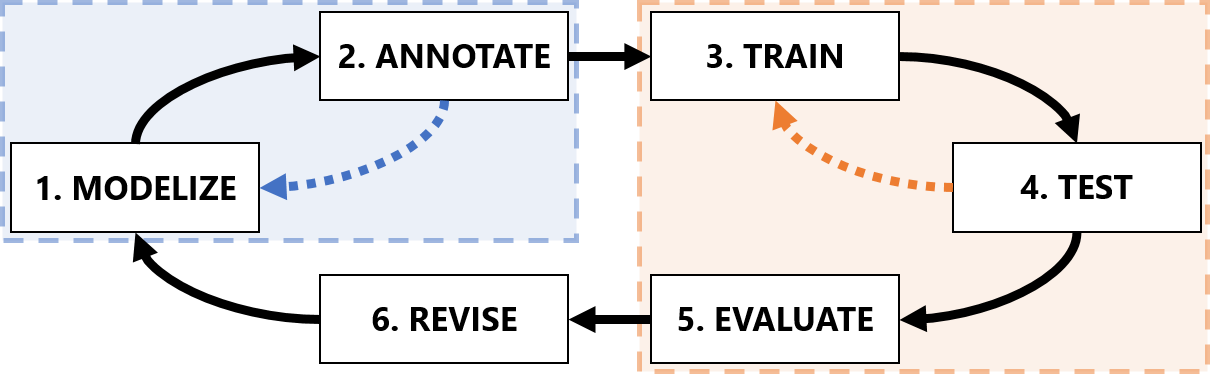
\includegraphics[width=0.95\textwidth]{figures/etatdelart-pustejovsky-2012-cycle-matter-mama-tt}
			\caption{
				Cycle \texttt{MATTER} structurant un projet d'annotation en six étapes principales: \textit{\textbf{M}odelize}, \textit{\textbf{A}nnotate}, \textit{\textbf{T}rain}, \textit{\textbf{T}est}, \textit{\textbf{E}valuate} et \textit{\textbf{R}evise}. \\
				Le carré bleu identifie le mini-cycle \texttt{MAMA} durant lequel la modélisation est adaptée en cours d'annotation,
				et le carré orange identifie le mini-cycle \textit{\textbf{T}rain}-\textit{\textbf{T}est} lors de la conception du modèle.
			}
			\label{figure:2.2.1-ORGANISATION-ANNOTATION-ETAPES-CLES-MATTER}
		\end{figure}
		%
		\begin{leftBarAuthorOpinion}
			Nous conseillons \cite{finlayson-erjavec:2016:overview-annotation-creation} pour son excellente revue de littérature qui détaille pas à pas le cycle \texttt{MATTER} tout en dressant la liste des points importants importants de chacune des étapes.
		\end{leftBarAuthorOpinion}
		
		%%% 2.2.1.A. Concevoir la base d'apprentissage (\textbf{M}odelize}, \textit{\textbf{A}nnotate}).
		\subsubsection{Concevoir la base d'apprentissage (\textit{\textbf{M}odelize}, \textit{\textbf{A}nnotate}).}
		\label{section:2.2.1.A-ORGANISATION-ANNOTATION-ETAPES-CLES-MODELIZE-ANNOTATE}
		
			%%% a. Collecte de données.
			Pour obtenir un bon modèle de \textit{Machine Learning}, il faut avoir une base d’apprentissage de qualité.
			Comme nous l'avons dit précédemment, cela commence par disposer d'un ensemble de données d'exemples qui représente fidèlement les différentes facettes du problème à modéliser (voir \textsc{Section~\ref{section:2.3.1.A-DEFIS-ANNOTATION-ASPECT-DONNEES-REPRESENTATIVITE}}).
			Une phase de \texttt{collecte} de données est alors organisée : cette collecte peut se baser sur des extractions de bases de données ou de sites internet à disposition, sur des enquêtes réalisées après d'utilisateurs finaux, ou encore sur les avis éclairés d'experts du problème.
			Certaines données peuvent aussi être artificiellement créées afin de compléter la collecte pour les aspects du problème difficile à observer.
			Une fois la collecte terminée, ces données brutes ont besoin d'être annotées pour pouvoir être exploitées. \\
			
			%%% b. Modelisation des données.
			
			% Importance de la modélisation.
			Afin de garantir la qualité de cette labellisation, \textbf{il est important de ne pas précipiter la tâche d'annotation}.
			En effet, l'objectif de cette tâche peut considérablement changer en fonction du phénomène à décrire, des données à disposition et de la finalité du modèle de \textit{Machine Learning} à entraîner.
			Il est donc fortement conseillé de bien \textbf{modéliser le problème}, c'est-à-dire de définir l'objectif de l'annotation, de clarifier en amont les modalités et les attendus de de cette tâche, et de préciser les règles que devront suivre les opérateurs.
			
			% Modélisation vs Spécification, Guide d'annotation et exemple.
			\cite{pustejovsky-stubbs:2012:natural-language-annotation} précisent notamment deux concepts importants de cette phase :
			\begin{itemize}
				\item la \textbf{modélisation} du problème, représentation de manière abstraite l'objectif à atteindre et décrivant ainsi la logique générale de l'annotation dans un \textit{schéma d'annotation} ;
				\item les \textbf{spécifications}, compilant dans un \textit{guide d'annotation} l'ensemble des règles concrètes à respecter pour mettre en application la modélisation.
			\end{itemize}
			Pour résumer cette distinction, la modélisation représente \textit{quoi} annoter (\textit{objectif, définition, valeurs possibles, ...}) alors que les spécifications décrivent \textit{comment} annoter (\textit{règles d'attribution, exemples et contre-exemple, règles de format, ...}).
			%
			\begin{leftBarExamples}
				% Exemple littérature.
				\cite{perrotin-etal:2018:annotation-actes-dialogue}, s'intéressant à la classification des conversations d'assistance en ligne en actes de dialogues, décrit son guide d'annotation dans \cite{asher-etal:2017:manuel-annotation-actes}.
				On y retrouve (1) la modélisation avec la présentation des étiquettes possibles à annoter, et (2) les spécifications avec les définitions concrètes, des exemples, des restrictions d'attribution, et la gestion des données non pertinentes. \\
				% Exemple BD.
				Dans nos exemples précédents (cf. \textsc{Section~\ref{section:2.1.2.B-PRESENTATION-ANNOTATION-EXEMPLES-CLASSIFICATION}}), nous avions modélisé le problème de classification de l'état d'une bande dessinée en quatre classes : "\texttt{Mauvais état}", "\texttt{Bon état}", "\texttt{Très bon état}", "\texttt{Neuf}".
				Il faudrait désormais rédiger les spécifications avec des définitions concrètes et quelques exemples  pour guider un annotateur, notamment pour l'aider à distinguer "\texttt{Bon état}" de "\texttt{Très bon état}".
			\end{leftBarExamples}
			
			% Quelques points importants sur la modélisation et exemples.
			Bien entendu, il n'est pas toujours facile de modéliser un problème ni de rédiger un guide d'annotation adéquat.
			Nous reviendrons plus tard sur les caractéristiques de cette tâche pouvant introduire de la complexité (voir \textsc{Section~\ref{section:2.3-DEFIS-ANNOTATION}}), mais il est important de souligner d'emblée les points élémentaires suivants :
			\begin{itemize}
				\item le besoin d'\textit{inter-opérabilité} et de \textit{ré-utilisabilité} : un projet d'annotation est toujours un investissement coûteux, il serait donc regrettable de perdre ou de ne pas pourvoir ré-utiliser ces données après ce projet.
				Par conséquent, il faut réfléchir au format des données ainsi qu'aux types de détails à fournir pour être sûr de pouvoir toujours exploiter les données si la modélisation évolue légèrement ou si un futur projet désire en bénéficier ;
				\item la balance entre \textit{généralité} et \textit{spécificité} : le niveau de détail requis dépend sans conteste du problème à modéliser : annoter trop peu de détail ne permet pas d'exploiter les données, mais en annoter trop peut rapidement complexifier la tâche et introduire des erreurs.
				Il faut donc trouver le juste milieu pour réaliser un travail de qualité qui ne soit pas trop pénible.
			\end{itemize}
			%
			\begin{leftBarExamples}
				Dans la classification de langue exposée en \textsc{Section~\ref{section:2.1.2.B-PRESENTATION-ANNOTATION-EXEMPLES-CLASSIFICATION}}, nous y avons annoté chaque texte grâce à trois classes : "\texttt{Français}", "\texttt{Anglais}" et "\texttt{Allemand}".
				\begin{itemize}
					% Exemple inter-opérabilité et de ré-utilisabilité.
					\item par soucis d'\textit{inter-opérabilité}, nous pourrions plutôt utiliser la norme ISO 639-3 (\cite{international-organization-for-standardization:2007:codes-representation-names}), soit les code "\texttt{fra}", "\texttt{eng}" et "\texttt{deu}", afin de standardiser l'annotation et ainsi pouvoir partager plus facilement les données labellisées avec d'autres projets ;
					% Exemple généralité et spécificité.
					\item afin de présenter un cas simple, nous avions proposé un modèle avec trois langues communes pour une bande dessinée d'origine belge.
					Toutefois, nous aurions pu \textit{spécialiser} davantage notre modèle en fonction des variations régionales en prenant en compte le Corse ("\texttt{cos}") ou le Wallon ("\texttt{wln}").
					Cette distinction peut être essentielle pour certaines saga publiées dans ces langues (comme \texttt{Astérix \& Obélix}), mais peut simplement être une source de confusion pour les autres (comme \texttt{Lucky Luke}).
				\end{itemize}
			\end{leftBarExamples}
			
			% Aide à la formalisation.
			\begin{leftBarInformation}
				Pour aider à concevoir le guide d'annotation et afin de se poser les bonnes questions, \cite{dipper-etal:2004:useradaptive-annotation-guidelines} dresse une liste de définitions et de recommandations à prendre en considération.
				Bien que ces conseils soient issus du traitement de données linguistiques, ils permettent d'identifier les sections importantes d'un guide d'annotation en fonction des attentes des différents acteurs de l'annotation (\textit{l'auteur, l'annotateur, l'explorateur de données, ...}) et de les rédiger en suivants certaines règles simples (\textit{introduire les objectifs, ordonner les règles par complexité, traiter en premier les cas par défaut, trier les valeurs des variables catégorielles par ordre alphabétiques, ...}).
				Des exemples reconnus pour leur bonne conception y sont notamment cités si vous avez besoin de référence pour concevoir votre propre guide.
			\end{leftBarInformation}
			
			
			%%% c. Annotation
			
			% Annotation en tant que telle.
			Lorsque le guide d'annotation est rédigé, la \textbf{phase de labellisation} peut commencer.
			Cette tâche est traditionnellement réalisée par un groupe d'experts choisi en fonction de leur connaissance sur le problème à caractériser (\textit{dans nos exemples sur les bandes dessinées, ce serait plutôt des libraires ou des collectionneurs}).
			Après leur avoir expliqué l'objectif de leur travail et partagé les règles de labellisation contenues dans le guide, les annotateurs se partagent les données et réalisent chacun une partie du corpus d'apprentissage.
			
			%%% d. Mini-cycle MAMA.
			
			\begin{leftBarInformation}
				% La théorie rencontre le réel.
				C'est généralement à ce stade que la théorie rencontre la pratique : certaines règles d'annotation peuvent difficilement être applicables, certains données peuvent être ambiguës ou hors-sujet, et deux annotateurs peuvent aussi avoir des avis différents sur l'annotation la plus adéquate.
				Il est aussi important de rappeler que l’annotation est un acte d'interprétation, et que les données sont donc labellisées par un humain dont l'avis n'est pas infaillible. 
				\cite{pustejovsky-stubbs:2012:natural-language-annotation} introduisent donc le premier sous-cycle \texttt{MAMA} en référence à la boucle entre \textit{\textbf{M}odelize} et \textit{\textbf{A}nnotate} qui peut avoir lieu tant que le guide d'annotation n'est pas adapté aux données manipulées ou que différents points de vues opposent les annotateurs.
				
				% Exemple.
				Par exemple, lors de l'annotation de la transcription audio en \textsc{Section~\ref{section:2.1.2.D-PRESENTATION-ANNOTATION-EXEMPLES-TRANSCRIPTION}}, il peut y avoir une voix principale accompagnée de plusieurs voix en arrière plan : une première adaptation du guide serait de clarifier si ces voix secondaires doivent être transcrites ou ignorées, voire si l'audio entier doit être considéré comme inexploitable.
				La réponse à cette question dépend bien entendu du phénomène à décrire et de l'objectif du modèle de \textit{Machine Learning} à entraîner : dans notre cas, nous pourrions probablement annoter uniquement la voix principale et ignorer l'audio si le bruit gène la compréhension.
			\end{leftBarInformation}
			
			%%% Finalité : la base d'apprentissage.
			À la fin de l'annotation (ou du cycle \texttt{MAMA}), le corpus d'entraînement est disponible pour concevoir un modèle de \textit{Machine Learning}.
		
		
		%%% 2.2.1.B. Concevoir le modèle (\textit{\textbf{T}rain}, \textit{\textbf{T}est}, \textit{\textbf{E}valuate}).
		\subsubsection{Concevoir le modèle (\textit{\textbf{T}rain}, \textit{\textbf{T}est}, \textit{\textbf{E}valuate}).}
		\label{section:2.2.1.B-ORGANISATION-ANNOTATION-ETAPES-CLES-TRAIN-TEST}
			
			%%% Apprentissage statistiques et importance du test.
			La phase d'entraînement du modèle est l'étape centrale de l'apprentissage automatique.
			Toutefois, comme l'apprentissage se base sur des méthodes statistiques, il est important d'introduire une phase de test et d'évaluation pour s'assurer des performances du modèle obtenu.
			Il est donc courant de considérer une boucle de raffinement du modèle tant que les performances n'ont pas atteint un seuil acceptable.
			
			%%% Train/Dev/Test.
			En pratique, il est d'usage de \textbf{créer trois jeux de données} à partir de la base d'apprentissage qui vient d'être annotée :
			\begin{itemize}
				% Train.
				\item le jeu d'\texttt{entraînement} :
				c'est sur cette partie des données que le modèle de \textit{Machine Learning} est conçu ;
				% Test.
				\item le jeu de \texttt{développement} (ou de validation) :
				le modèle entraîné est évalué sur ce jeu de donnée pour étudier son comportement, identifier ses forces et ses faiblesses, et ainsi permettre de le comparer à d'autres modèles entraînés pour cette même tâche ;
				% Dev.
				\item le jeu de \texttt{test} :
				le modèle retenu est évalué sur ce jeu de test pour déterminer ses performances réelles.
			\end{itemize}
			% \cite{van-der-goot:2021:we-need-talk}: définir un train/tune/dev/test
			
			%%% Evaluate.
			Ainsi, le modèle représente la connaissance présente dans le jeu \texttt{entraînement}, il est étudié puis affiné grâce au jeu de \texttt{développement}, et est finalement jugé en fonction de ses performances sur le jeu de \texttt{test}.
			Il est encore une fois difficile d'être exhaustif sur les analyses et les métriques à considérer car elles dépendent fortement du type de problème que le modèle tente de résoudre.
			Une métrique basique est l'\texttt{Accuracy} (ou taux de bonne prédiction), décrivant simplement le nombre de fois que le modèle a fait une bonne proposition sur l'ensemble du test.
			Suivant le problème et le type de données, d'autres métriques usuelles peuvent être utilisées comme le \texttt{MSE} (\textit{Mean Squared Error}) pour la prédiction de variables numérique (voir \cite{wallach-goffinet:1987:mean-squared-error}), le \texttt{f1-score} pour les variables catégorielles (voir \cite{sasaki:2007:truth-fmeasure}) ou le \texttt{WER} (\textit{Word Error Rate}) pour la transcription de textes (voir \cite{mccowan-etal:2005:use-information-retrieval}).
			Dans tous les cas, une règle d'or est de bien tenir à l'écart le jeu de test des deux autres jeux de données et qu'il ne soit pas utilisé dans la phase de développement pour éviter tout biais de sur-apprentissage\footnote{
				Pour plus de détails sur le sur-apprentissage: voir \cite{collins:2017:chapter-overfitting}
			}.

			%%% Finalité : le modèle et se sperformances.
			À la fin de ce cycle, le modèle de \textit{Machine Learning} est à disposition, et ses performances théoriques sont celles obtenues sur le jeu de test.
		
		%%% 2.2.1.C. Revoir la base d'apprentissage (\textit{\textbf{R}evise}).
		\subsubsection{Revoir la base d'apprentissage (\textit{\textbf{R}evise}).}
		\label{section:2.2.1.C-ORGANISATION-ANNOTATION-ETAPES-CLES-REVISE}
		
			% Besoin de réviser.
			Pour terminer cette boucle, il est parfois nécessaire d'envisager de corriger son modèle en remettant en cause la modélisation du problème et l'annotation des données.
			\cite{voormann-gut:2008:agile-corpus-creationa} formalisait en effet ce besoin de réviser la conception d'une base d'apprentissage en observant les lacunes du modèle obtenu, et \cite{pustejovsky-stubbs:2012:natural-language-annotation} évoque certaines révisions nécessaires de la modélisation dès la phase d'annotation (voir sous-cycle \texttt{MAMA} dans la \textsc{Figure~\ref{figure:2.2.1-ORGANISATION-ANNOTATION-ETAPES-CLES-MATTER}}).
			
			% Identifier un besoin de réviser.
			Divers pistes peuvent mener à une évolution de la base d'apprentissage :
			\begin{itemize}
				\item le modèle de \textit{Machine Learning} peut avoir de mauvaise performances, malgré son affinage lors de la phase de développement, ou peut manquer d'adaptabilité sur des données réelles ;
				\item la modélisation ou l'annotation peuvent devenir obsolète car le phénomène modélisé évolue dans le temps ;
				\item un cas d'usage non identifié jusqu'à présent nécessite de nouvelles données pour être pris en compte ;
				\item le modèle peut ne pas convenir aux utilisateurs finaux par manque d'ergonomie ou à cause d'une utilisation non prévue initialement ;
				\item ou encore, un nouvel algorithme de \textit{Machine Learning} a priori plus performant requiert une modélisation différente pour traiter le problème.
			\end{itemize}
			%
			\begin{leftBarExamples}
				% Exemple Inflation prix
				Pour illustrer nos propos, prenons la tâche d'estimation du prix d'une bande dessinée (cf. \textsc{Section~\ref{section:2.1.2.A-PRESENTATION-ANNOTATION-EXEMPLES-REGRESSION}}) : il se peut que les prix annoté sur les transactions ne soient plus d'actualité à cause de l'inflation, et que les données doivent être ré-annotées pour prendre en compte les nouvelles valeurs du marché.
				
				% Exemple ajouter une classe.
				D'autre part, la modélisation en tant que telle peut aussi être impacté : par exemple, dans le cadre de la classification de l'état d'une bande dessinée à partir d'une photo (cf. \textsc{Section~\ref{section:2.1.2.B-PRESENTATION-ANNOTATION-EXEMPLES-CLASSIFICATION}}), on pourrait constater à l'usage qu'il manque une catégorie "\texttt{Très mauvais état}" nécessaire pour trier d’emblée toute \texttt{BD} indigne à la vente.
				
				% Exemple OCR.
				Enfin, il est possible que le modèle se comporte mal sur certaines données.
				Par exemple lors de l'identification d'une bande dessinée à partir de sa couverture (cf. \textsc{Section~\ref{section:2.1.2.C-PRESENTATION-ANNOTATION-EXEMPLES-EXTRACTION}}), certains textes du décors pourrait être extrait à tord (comme le texte de la pancarte \textguillemets{\textit{Saloon}} dans la \textsc{Figure~\ref{figure:2.1.2.C-PRESENTATION-ANNOTATION-EXEMPLES-IMAGE-OCR}}).
				Il faudra peut-être adapter l'annotation pour identifier les textes à ne pas extraire (avec une classe de rebus par exemple).
			\end{leftBarExamples}
			
			% Conclusion.
			Nous bouclons ainsi le cycle \texttt{MATTER} qui préfigure le besoin d'une amélioration continue d'un modèle de \textit{Machine Learning} pour que celui-ci soit le plus adapté à son environnement d'utilisation.
	
	
	%%%
	%%% Subsection 2.2.2: Portraits des acteurs intervenant sur un projet d'annotation.
	%%%
	\subsection{Portraits des acteurs intervenant sur un projet d'annotation}
	\label{section:2.2.2-ORGANISATION-ANNOTATION-ACTEURS}
	
		% Introduction: grande diversité de métiers.
		Au cours du cycle \texttt{MATTER}, nous pouvons constater que divers acteurs interviennent pour concevoir la base d'apprentissage et entraîner un modèle de \textit{Machine Learning}.
		Cette diversité de métiers qui gravitent autour du traitement automatique des données semble difficile à détailler, tant à cause de leur grand nombre que de leurs subtiles différences.
		Pour avoir un aperçu, vous pouvez consulter les offres d'emplois du marché actuel (voir \cite{team-datascientest:2022:metiers-data-mieux} ou \cite{databird:2023:10-metiers-data}) ou certaines formations professionnelles (voir \cite{isoz:2017:decouvrir-metiers-data}) pour pouvoir faire la distinction entre \textit{data scientist}, \textit{data analyst}, \textit{data librarian}, \textit{data journalist}, \textit{data architect}, \textit{data engineer}, \textit{data steward}, \textit{data archivist}, ou encore \textit{machine learning engineer}...
		
		% Approche par compétences.
		Afin d'avoir une approche moins commerciale de ces métiers, nous proposons plutôt de dresser les compétences requises au diverses phases du cycle, à l'image de \cite{radovilsky-etal:2018:skills-requirements-business} qui présente les acteurs de la science des données grâce à quatre groupes de compétences :
		\begin{enumerate}
			% Business expert.
			\item les compétences \textbf{métiers} : elles sont liées aux connaissances et à l'expertise sur le phénomène à modéliser ou le problème à résoudre.
			Ce sont grâce à ces compétences qu'un acteur peut être apte à annoter une donnée ou à qualifier la pertinence de la prédiction d'un modèle de \textit{Machine Learning}.
			Les métier(s) associé(s) sont : l'\texttt{expert métier} (\textit{business expert}) ;
			% Data analyst.
			\item les compétences \textbf{analytiques} : elles concernent entre autres la modélisation du problème, la gestion des données, et les analyses statistiques sur les biais et les performances.
			Ce sont grâce à ses compétences qu'un acteur peut concevoir le guide d'annotation, estimer le taux d'accord inter-annotateurs, ou encore réaliser l'évaluation statistique d'un modèle de \textit{Machine Learning}.
			Les métier(s) associé(s) sont : l'\texttt{analyste des données} (\textit{data analyst}) ou le \texttt{scientifique des données} (\textit{data scientist}) ;
			% Data scientist.
			\item les compétences \textbf{techniques} : elles portent sur l'ingénierie autour du modèle de \textit{Machine Learning}, comme le choix du meilleur algorithme d'entraînement et réglage fin des hyper-paramètres, l'archivage des différentes versions du modèle ainsi que son déploiement dans un environnement de production.
			Les métier(s) associé(s) sont : le \texttt{scientifique des données} (\textit{data scientist}), l'\texttt{ingénieur en Machine Learning} (\textit{Machine Learning Engineer}) ou l'\texttt{architecte des des données} (\textit{data architecte}) ;
			% Projet leader.
			\item et les compétences en \textbf{gestion} ou en \textbf{communication} : elles permettent d'aborder le cadrage du projet et la définition des objectifs, ainsi que diverses aptitudes transverses comme l'établissement de rapports, la gestion de projet, la vérification des normes, ...
			Les métier(s) associé(s) sont : le \texttt{chef de projet} (\textit{project leader}) ou le \texttt{responsable de la protection des données} (\textit{data protection officer}).
		\end{enumerate}
		\begin{leftBarInformation}
			On peut compléter cette vision par compétences avec la vision donnée par \cite{fort:2017:experts-ou-foule}, selon laquelle il y a trois types d'experts lors d'un projet d'annotation :
			\begin{itemize}
				\item les \textbf{experts du corpus} de données, ayant par exemple les connaissances sur les bandes dessinées, s'approchant donc de compétences \texttt{métiers} ;
				\item les \textbf{experts de l'annotation}, ayant par exemple les connaissances sur l'annotation de textes dans une image, s'approchant donc de compétences \texttt{analytiques} ;
				\item et les \textbf{experts de la tâche} de \textit{Machine Learning}, ayant par exemple les connaissances sur les techniques d'\texttt{OCR}, s'approchant donc des compétences \texttt{techniques}.
			\end{itemize}
		\end{leftBarInformation}
		
		% Application au cycle \texttt{MATER}.
		Ainsi, durant le cycle \texttt{MATTER}, nous pouvons voir les compétences ci-dessus se compléter :
		\begin{enumerate}
			% Concevoir la base d'apprentissage.
			\item la conception de la \textbf{base d'apprentissage} (étapes \textit{\textbf{M}odelize} et \textit{\textbf{A}nnotate}) nécessite :
			\begin{itemize}
				\item des compétences de \texttt{gestion} pour cadrer l'objectif du modèle à entraîner, et ainsi définir l'objectif auquel doit répondre l'annotation de données ;
				\item des compétences \texttt{analytiques} pour proposer une modélisation stable du phénomène et un guide d'annotation précis pour limiter les biais de conception ;
				\item des compétences \texttt{métiers} pour vérifier que la proposition de modélisation est pertinente vis-à-vis du cas d'usage, mais aussi pour réaliser l'annotation des données.
			\end{itemize}
			% Concevoir le modèle.
			\item la conception du \textbf{modèle de \textit{Machine Learning}} (étapes \textit{\textbf{T}rain}, \textit{\textbf{T}est}, \textit{\textbf{E}valuate}) nécessite :
			\begin{itemize}
				\item des compétences \texttt{analytiques} pour gérer les jeux de données (\textit{entraînement, développement, test}) et évaluer les performances statistiques du modèle ;
				\item des compétences \texttt{techniques} pour manipuler l'écosystème de développement du modèle, régler les hyper-paramètres, versionner les changements, et planifier la distribution du modèle ;
				\item des compétences de \texttt{gestion} pour s'assurer du respect des normes et des caractères privée ou confidentielle de certaines données.
			\end{itemize}
			% Revoir la base d'apprentissage
			\item la \textbf{révision} de la base d'apprentissage (étape \textit{\textbf{R}evise}) nécessite :
			\begin{itemize}
				\item des compétences \texttt{métiers} pour identifier le manque de pertinence du modèle vis-à-vis de certains cas d'usage ;
				\item des compétences \texttt{analytiques} pour disserter des performances réelles du modèle face à des données de production et remettre en question les précédents choix de modélisation pour espérer améliorer le modèle.
			\end{itemize}
		\end{enumerate}
		
		% Remarque sur la distance entre métier et technique.
		On notera que les compétences transverses de \textbf{gestion} ou \textbf{communication} ne sont pas spécifiques à une étape du cycle \texttt{MATTER} (\textit{le cadrage, la gestion de projet et l'établissement de rapports étant réalisés tout au long du projet}), alors que les compétences \texttt{métier} et \texttt{techniques} n'interviennent généralement pas au même moment du cycle : autrement dit, des experts métiers croisent rarement des experts techniques et ne partagent donc que très rarement leurs connaissances.
	
	
	%%%
	%%% Subsection 2.2.3: Choix du logiciel d'annotation.
	%%%
	\subsection{Choix du logiciel d'annotation}
	\label{section:2.2.3-ORGANISATION-ANNOTATION-LOGICIELS}
	
		% Introduction: besoin d'un outil d'annotation.
		Pour terminer la description de l'organisation d'un projet d'annotation, attardons nous sur le choix du logiciel à utiliser pour labelliser les données.
		En effet, une diversité d'applications existent pour répondre aux besoins des annotateurs, mais il est important de noter que l'absence de certaines fonctionnalités essentielles risque de gêner le projet d'annotation, soit par l'introduction de biais, soit à cause de son manque d'inter-opérabilité avec d'autres tâches d'analyses ou d'annotation.
		
		% Liste des fonctionnalités importantes.
		Nous faisons référence à \cite{finlayson-erjavec:2016:overview-annotation-creation} pour dresser ci-dessous une liste des fonctionnalités principales (voire essentielles) d'un logiciel d'annotation.
		Pour simplifier la lecture, nous proposons de regrouper ces fonctionnalités dans les catégories suivantes :
		\begin{itemize}
			% Répondre à la \textbf{besoin d'annotation}.
			\item répondre à la \textbf{besoin d'annotation} :
				cette fonctionnalité est bien entendu obligatoire, car un logiciel ne permettant pas d'annoter vos données ne vous sera d'aucune utilité.
				Cette remarque semble être une évidence, mais nous nous permettons aussi d'étendre l’avertissement aux logiciels n'étant pas destinés à votre besoin d'annotation mais qui peuvent être détournés pour y répondre indirectement : de telles contournements peuvent introduire des biais et offrent généralement une expérience utilisateur assez médiocre ;
			% Intégrer le \texbf{guide d'annotation}.
			\item intégrer le \textbf{guide d'annotation} :
				ce livrable issu de la phase de modélisation du cycle \texttt{MATTER} doit être facilement accessible par les annotateurs car il contient la documentation et les instructions à appliquer lors de la labellisation.
				Les logiciels permettant d'intégrer directement ces définitions (\textit{avec exemples et contre-exemples}) ainsi que les règles d'annotation (\textit{comme les labels mutuellement exclusifs, les détails obligatoires, ...}) ont donc un net avantage ergonomique pour respecter la modélisation définie et ainsi garantir la qualité de la base d'apprentissage ; 
			% Autoriser l'\textbf{annotation multiple}.
			\item autoriser l'\textbf{annotation multiple} et l'\textbf{annotation multi-modale}: 
				il est fréquent de devoir annoter plusieurs une même donnée suivant des modélisations ou des paradigmes différents pour répondre à plusieurs cas d'usage (\textit{en prenant l'exemple de l'annotation d'images, on peut détourer les objets présents, identifier les textes inscrits, proposer une ou plusieurs catégories générales, proposer une description textuelle, ...}) ou encore de devoir annoter des données de natures différentes (\textit{en combinant texte, image et voix comme dans l'annotation des sous-titres d'une vidéo}).
				Les logiciels permettant ainsi de labelliser plusieurs informations et de manipuler plusieurs types de données sont donc plus facilement réutilisables et permettent de centraliser les annotations ;
			% Evaluer la \textbf{qualité de l'annotation}.
			\item évaluer la \textbf{qualité de l'annotation} :
				les erreurs d'annotation et les divergences d'opinions sur la modélisation sont inévitables.
				Il est donc appréciable de pouvoir les identifier, soit sur la base d'une comparaison directe entre deux annotateurs, soit en comparant avec l'annotation la plus probable issue d'une base de référence.
				Il peut aussi être intéressant de pouvoir calculer les scores d'accord inter-annotateurs sur un même échantillon de données pour estimer la qualité de la base d'apprentissage, de pouvoir corriger les erreurs lors de revues ou encore de trancher les cas de conflits apparent lors d'avis discordants ;
			% Permettre l'\textbf{inter-opérabilité} technique.
			\item permettre l'\textbf{inter-opérabilité} technique :
				il est toujours frustrant de ne pas pouvoir réutiliser des annotations d'un projet à l'autre car le format de stockage n'est pas compatible.
				Les logiciels prenant donc en considération plusieurs format de données (\textit{\texttt{PNG}/\texttt{JPG}, \texttt{MP3}/\texttt{WAV}, \texttt{XLSX}/\texttt{XML}/\texttt{JSON}, ...}) et respectant les standards de la tâche d'annotation lors des imports et exports sont donc à privilégier.
				De plus, il est conseillé de ne pas écrire directement les annotation dans les données (\textguillemets{\textit{\textbf{[Lucky Luke]}{\textcolor{colorDarkPastelRed}{\texttt{/(personnage)}}}, le \textbf{[cow-boy]}{\textcolor{colorDarkPastelPurple}{\texttt{/(métier)}}} solitaire, a ...}}), mais de les stocker dans des fichiers séparés pour garder une meilleure gestion et permettre les annotations multiples ;
			% Gérer le \textbf{flux de travail} et le \textbf{suivi de projet}.
			\item gérer le \textbf{flux de travail} et le \textbf{suivi de projet} :
				certaines fonctionnalités simples sont nécessaires à l'organisation de l'équipe d'annotation.
				Cela peut comprendre la répartition de la charge de travail, l'historisation des changements pour permettre les retours arrières, la possibilité d'émettre des appels d'aide ou d'écrire des commentaires sur les choix d'annotation, ou encore l'accompagnement des nouveaux annotateurs lors de leur monté en compétence ;
			% Favoriser le \textbf{confort de l'annotateur}.
			\item favoriser le \textbf{confort de l'annotateur} :
				le logiciel choisi sera utilisé au quotidien par l'équipe d'annotation, il semble donc essentiel de leur offrir une expérience utilisateur agréable pour réaliser leur tâche.
				Cela peut passer par une customisation de l'interface utilisateur afin d'être adapter à l'objectif d'annotation et par le paramétrage de raccourcis claviers.
				Simplifier l'accès et l'installation du logiciel peut aussi s'avérer utile pour favoriser son adoption, en favorisant par exemple les applications web permettant plus facilement le travail collaboratif ;
			% Permettre des \texbf{annotations et d'analyses avancées}.
			\item permettre des \textbf{annotations et d'analyses avancées} :
				la littérature scientifique regorge de techniques pouvant assister un annotateur dans son travail (\textit{pré-annotation, apprentissage actif, visualisation, interaction, ...}).
				Nous détaillons plusieurs de ces techniques dans la \textsc{Section~\ref{section:2.3-DEFIS-ANNOTATION}}.
		\end{itemize}
		
		% Quelques exemples.
		Considérant la diversité de cas d'usage d'annotation, une liste exhaustive des outils de labellisation n'est bien entendu pas possible.
		Nous tenons toutefois à présenter quelques exemples illustrés dans la \textsc{Figure~\ref{figure:2.2.3-ORGANISATION-ANNOTATION-LOGICIELS}}.
		%
		\begin{figure}[!htb]
			\centering
			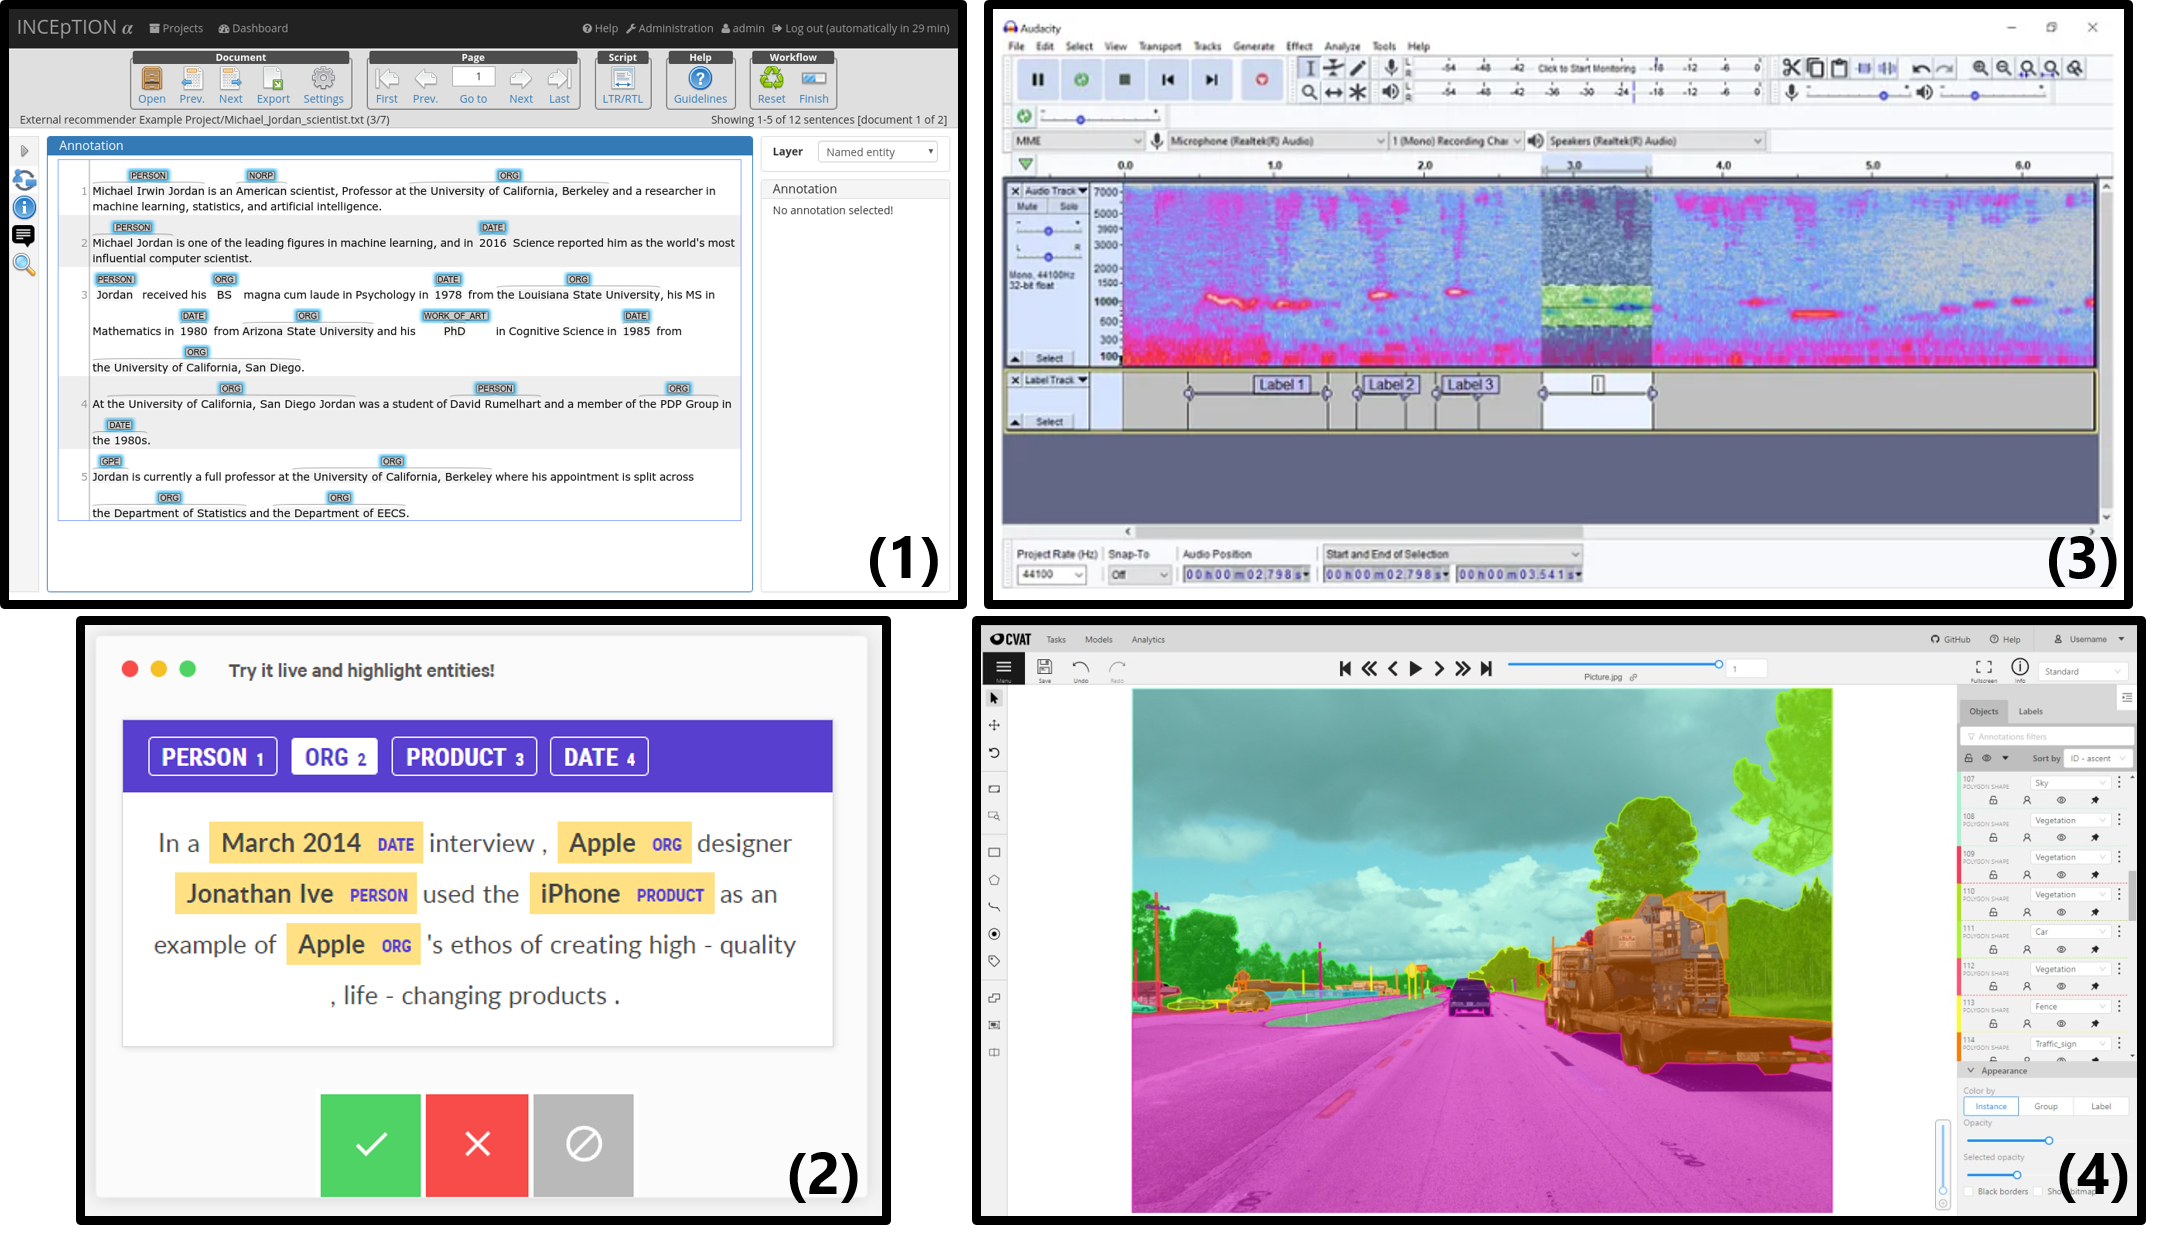
\includegraphics[width=0.95\textwidth]{figures/etatdelart-logiciel-exemples}
			\caption{
				Quatre exemples d'outils d'annotation :
				\textbf{(1)} \texttt{INCEpTION} pour le texte (\cite{klie-etal:2018:inception-platform-machineassisted}),
				\textbf{(2)} \texttt{prodigy} pour le texte ou l'image (\cite{montani-honnibal:2017:prodigy-modern-scriptable}),
				\textbf{(3)} \texttt{Audacity} pour l'audio (\cite{audacity-team:2000:audacity-free-audio}
				et \textbf{(4)} \texttt{CVAT} pour l'image (\cite{cvat.ai-corporation:2019:computer-vision-annotation}).
			}
			\label{figure:2.2.3-ORGANISATION-ANNOTATION-LOGICIELS}
		\end{figure}
		
		% Avis sur la sur-utilisation d'Excel.
		\begin{leftBarAuthorOpinion}
			De part notre expérience, nous constatons malheureusement que plusieurs projets industriels n'utilisent pas ou peu d'outils d'annotation dédiés, et se contentent plutôt d'outils rudimentaires comme des traitement de textes ou des tableurs tels que \texttt{Microsoft Excel} (\cite{microsoft-corporation:2018:microsoft-excel}).
			Une étude serait à mener pour étudier cette tendance et expliquer le manque d'intérêt porté aux outils spécialement conçus pour les tâches d'annotations.
			Peut-être que ces derniers s'adaptent mal aux particularités des divers projets industriels, expliquant ainsi l'utilisation d'outils simplistes mais flexibles. Ou alors est-ce par méconnaissance des difficultés et des bais potentiels de l'annotation que ces outils aux fonctionnalités avancées ne sont pas employés ?
		\end{leftBarAuthorOpinion}
	
	
	%%%
	%%% Subsection 2.2.4: Bilan concernant les nombreux défis de l'annotation.
	%%%
	\subsection{Bilan concernant l'organisation d'un projet d'annotation}
	\label{section:2.2.4-ORGANISATION-ANNOTATION-BILAN}
	
	%%%
	%%% Conclusion.
	%%%
	\begin{leftBarSummary}
		\begin{todolist}
			% MATTER.
			\item[\itemok] En général, un projet d'annotation est \textbf{organisé en cycle (\texttt{MATTER})} au cours duquel nous réalisons une modélisation abstraite des données que nous formalisons dans un guide (\textit{\textbf{M}odelize}), nous appliquons ce guide pour labelliser notre base d'apprentissage (\textit{\textbf{A}nnotate}), puis nous entraînons et testons un modèle de \textit{Machine Learning} (\textit{\textbf{T}rain}, \textit{\textbf{T}est} et \textit{\textbf{E}valuate}).
			Ensuite, l'évaluation du modèle peut mener à une révision de la modélisation des données en fonction des performances obtenues (\textit{\textbf{R}evise}) ;
			% Acteurs.
			\item[\itemok] Un tel projet d'annotation nécessite une \textbf{diversité de connaissances et de compétences} qui peuvent être réparties en quatre catégories : \texttt{métier}, \texttt{analytique}, \texttt{technique} et \texttt{gestion/communication} ;
			% Outils.
			\item[\itemok] Un tel projet nécessite aussi un \textbf{outil d'annotation dédié} possédant certaines fonctionnalités essentielles comme la possibilité d'\texttt{intégrer le guide} d'annotation, le besoin de \texttt{contrôler la qualité} des annotations, la capacité à réaliser des \texttt{annotation multiples ou multimodales}, ou encore l'assimilation d'éléments de \texttt{gestion de projet}.
		\end{todolist}
	\end{leftBarSummary}